\documentclass{article}

\usepackage{pdfpages}
\usepackage[utf8]{inputenc}
\usepackage{eurosym}
%\usepackage{fancyhdr}
%\pagestyle{fancy}

%
%Die eingegangenen Projektskizzen werden nach folgenden Kriterien bewertet:
%– Zielabdeckung: Das Vorhaben ist auf die Vermittlungsziele des Wissenschaftsjahres 2019 zugeschnitten (Berück-
%sichtigung der Handlungsfelder, Zielgruppen, Forschungsinhalte).
%– Fachliche Kompetenz: Der Antragsteller ist qualifiziert, das Vorhaben durchzuführen und verfügt über nachgewie-
%sene Expertise über das Themenfeld und/oder die Vermittlung des Themenfelds.
%– Schlüssigkeit und Konsistenz des Konzepts: Idee, Ziele, Budgetschätzung.
%– Kommunikative Ausrichtung und Wirksamkeit: Das Vorhaben wird von geeigneten Kommunikationsmaßnahmen be-
%gleitet, es ist öffentlichkeitswirksam und generiert voraussichtlich eine mediale Berichterstattung. Das Vorhaben wird
%kommunikativ in das Wissenschaftsjahr 2018 eingebunden und als Teil dessen wahrgenommen.
%– Innovation: Das Vorhaben ist innovativ und leistet einen Beitrag zur Weiterentwicklung der Wissenschaftskommuni-
%kation in Deutschland.
%– Überregionalität und Nachhaltigkeit: Das Vorhaben strahlt überregional aus und/oder kann übertragen bzw. nachgenutzt werden


\begin{document}


\begin{center}
%\vspace{-13cm}
{ \centering 
\includegraphics[width=10cm]{hsf.png} }

\vspace{-0.8cm}
\begin{figure*}[h!]
\centering
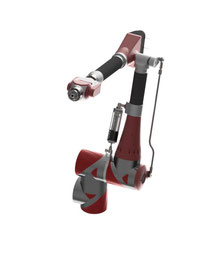
\includegraphics[width=0.6\textwidth]{arm.png}
\end{figure*}
\vspace{-1.8cm}

{\Huge\bf
PROJEKTSKIZZE: Lernen in Handarbeit
}
\\[2em]
\Large
{\bf Antragsteller:} Prof. Dr. Alexander Gepperth (HDR)\\
{\bf Adresse: } Fachbereich Angewandte Informatik der HAW Fulda\\
Leipzigerstr. 123, 36037 Fulda\\
{\bf Email: } alexander.gepperth@cs.hs-fulda.de\\
{\bf Telefon: } 0661 9640 3485\\
\vspace{0.5cm}

{\bf Projektdauer:} 9 Monate\\
\vspace{0.5cm}

{\bf Gesamtkosten:} 150.000\euro\\
\vspace{0.5cm}

{\bf Zuwendungsbedarf:} 150.000\euro\\
\vspace{0.5cm}

%{\bf Konsortium:} Assisted Living, Hilfe für Schwerbehinderte, Service-Robotik, 3D-Simulation
\end{center}
%\end{titlepage}
\newpage

\renewcommand{\thesection}{2}
\section{Antragsteller und assoziierte Partner}
blablabla

\renewcommand{\thesection}{3}
\section{Ausgangsfrage und Ziele des geplanten Vorhabens}
\subsection{Kurzzusammenfassung}
\subsection{Grundsätzliche Zielsetzung}
%
\renewcommand{\thesection}{4}
\section{Ausführliche Vorhabensbeschreibung}
gestenerkennung
Dissemination: MINTmachclub, Interaktionsformat, kinderuni,
interaktion mit gymnasialen Oberstufen, interface zur Java oder Python das per Rest die erkannte Geste ausgibt!
webseite
evtl einzelne Leute machen geste, dann halbe Klasse, dann ganze
visualisierung der ausgaben, sicherheit, konfidenz
visualisierung der Prototypen!
visualisierung was gelernt wurde: deep dreaming
ausgabe der berechnungsvotschrift als PDF
message: ist nur ein verfahren, keine Magie
lernen der einschränkungen: linek hand trainieren, rechte testen --> problem!


\renewcommand{\thesection}{5}
\section{Darstellung des Eigeninteresses/Eigenanteils}


\renewcommand{\thesection}{6}
\section{Nachhaltigkeit,Übertragbarkeit}
Arbeiten zum inkrementellen Lernen
Arbeiten an Gestenerkennung
Arbeiten an Sequenzerkennung
Einfache Datensammlung
Einsetzbarkeit in der Lehre

\renewcommand{\thesection}{7}
\section{Zeitplan}

\renewcommand{\thesection}{8}
\section{Finanzierungsplan}
mitarbeiter E11
Sensoren 1000€
Rechner 15000€
Depermässigung
2 Hiwis 9 Monate f Visualisierung und Infrastruktur
3 1T SSD-Festplatten für Daten: 2000€


\renewcommand{\refname}{}
\bibliographystyle{abbrv}
\bibliography{bib.bib}
%

\end{document}




